\documentclass[10pt, compress]{beamer}
\usetheme[conference=KoM,venue=Remote, date=28/04/2017, titleprogressbar, logo=RFX-logo]{Eurof}
\usepackage{listings,amsmath,multimedia, amssymb}
\usepackage{../beamerclass/tangocolors}
\usepackage{../beamerclass/rfxcolor}
% for drawing
\usepackage{pgf}
\usepackage{tikz}
\usetikzlibrary{arrows,shapes,backgrounds}
\usepackage{../beamerclass/onimage}
\usepackage[export]{adjustbox}
\usepackage{bm}
% for font
\usepackage[absolute,overlay]{textpos}
  \setlength{\TPHorizModule}{1mm}
  \setlength{\TPVertModule}{1mm}

\usepackage[style=nature,citestyle=authoryear-comp,defernumbers=true,maxnames=2,firstinits=true,
uniquename=init,backend=bibtex8,arxiv=abs,mcite]{biblatex}
\bibliography{biblio}
\renewcommand*{\bibfont}{\footnotesize}
\renewcommand*{\citesetup}{\footnotesize}
\usepackage[export]{adjustbox}
\makeatother
\mode<presentation>
\makeatletter
% add a macro that saves its argument
\newcommand{\footlineextra}[1]{\gdef\insertfootlineextra{#1}}
\newbox\footlineextrabox
% for reducing font on a single slide
\newcommand\Fontvi{\fontsize{8}{7.2}\selectfont}
\title{Topic 21: AUG experiment Week 17 Summary}
\date{28 April 2017}
\author[Topic 21 Scientific Team]{Topic 21 Scientific Team}
\begin{document}
\tikzstyle{every picture}+=[remember picture]
\maketitle

\begin{frame}{L-Mode}
\Fontvi
  \vspace{-1cm}
\begin{columns}
  \begin{column}{0.5\textwidth}
    \centering{\includegraphics[height=\textheight]{pdfbox/30269Shape}}
  \end{column}
  \begin{column}{0.5\textwidth}
    \begin{description}
      \item[\# 1] \textbf{EOC} Shape, 0.8MA, B$_{\phi}$ = -2.5 T, 0.5MW NBI heating,
        fueling as reference 30269, heating starting together with
        fueling
      \item[\# 2] Same density ramp and heating with I$_p$ = 0.61 MA,
        B$_{\phi}$ = -1.9T (reduced current with the same q$_{95}$)
      \item[\# 3] Same density ramp and heating with I$_p$ = 0.99 MA,
        B$_{\phi}$ = -3.1T (increased current with the same q$_{95}$)
      \item[\# 4] Same density ramp and heating B$_{\phi}$ = -2.5T and I$_{p}$ = 0.99 MA
      \item[\# 5] Same density ramp and heating B$_{\phi}$ = -2.5T and I$_{p}$ = 0.61 MA
    \end{description}
  
  \end{column}
\end{columns}
\end{frame}

\begin{frame}{Current scan at constant q$_95$}
  \Fontvi
  \begin{columns}
    \begin{column}{0.6\textwidth}
      \includegraphics[width=\textwidth]{../../Experiments/AUG/analysis/pdfbox/IpConstantq95_density}
    \end{column}
    \begin{column}{0.4\textwidth}
      \begin{itemize}
        \item Succesfull plasma current scan at constant
          q$_{95}$ (\# 34102,  34103, 34104).
        \item Actually at higher current $\overline{n}_e$ too
          high?
        \item It is true the flattening occurs earlier in density at
          lower current?
      \end{itemize}
    \end{column}
  \end{columns}
  
\end{frame}

\begin{frame}{Current scan at constant q$_95$}
  \Fontvi
  \begin{columns}
    \begin{column}{0.6\textwidth}
      \includegraphics[width=\textwidth]{../../Experiments/AUG/analysis/pdfbox/IpConstantBt_density}
    \end{column}
    \begin{column}{0.4\textwidth}
      \begin{itemize}
        \item At constant B$_t$ the flattening is less robust? Compare
          for example higher current at same density
      \end{itemize}
    \end{column}
  \end{columns}
\end{frame}


\begin{frame}{H-Mode}
\Fontvi
  \vspace{-1cm}
\begin{columns}
  \begin{column}{0.5\textwidth}
    \centering{\includegraphics[height=\textheight]{pdfbox/30269Shape}}
  \end{column}
  \begin{column}{0.5\textwidth}
    \begin{description}
      \item[\# 6] \textbf{EOC} Shape, repeat \# 33478 with P$_{NBI}$ =
        4MW, D$_2$ puffing starting at 4s up to 35$\times 10^{21}$ @
        6s. 1 Plunge of probe in safe position
      \item[\# 7] Repeat 6 adding N in feed-forward. Keep similar
        value as reference (since we are already increasing the fueling)
    \end{description}
  \end{column}
\end{columns}
\end{frame}

\begin{frame}{H-Mode}
  \Fontvi
  \begin{columns}
    \begin{column}{0.6\textwidth}
      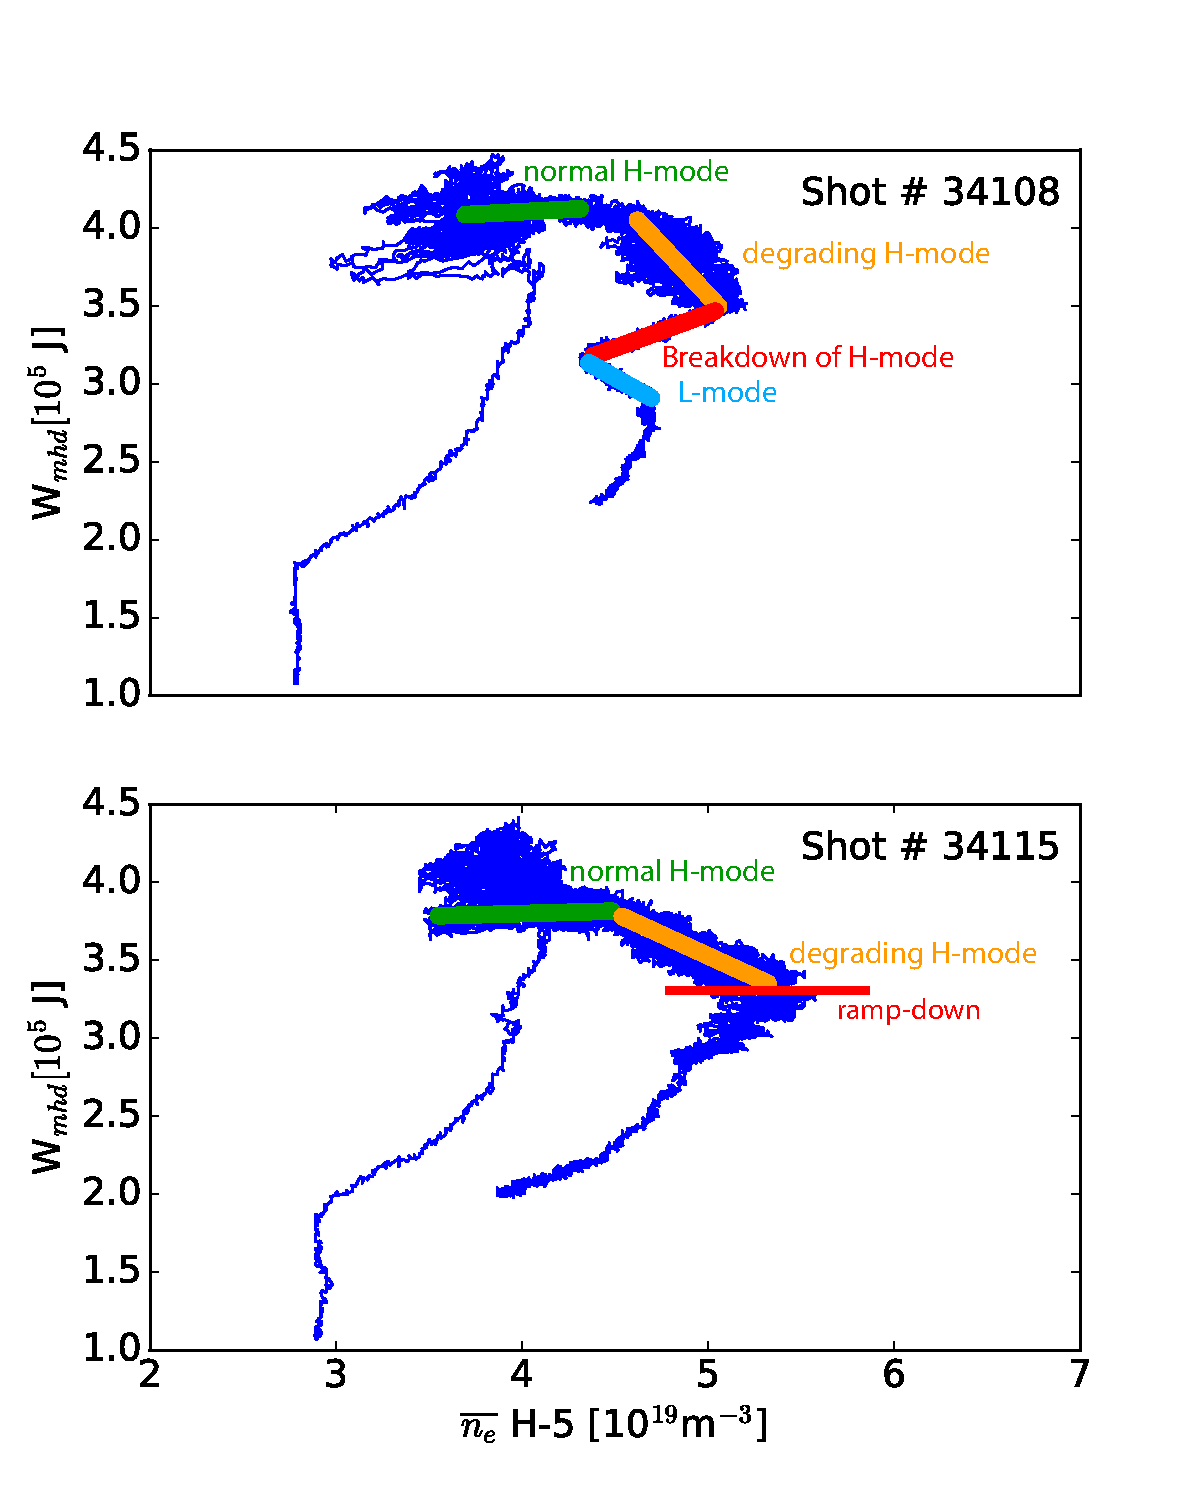
\includegraphics[width=\textwidth]{../../Experiments/AUG/analysis/pdfbox/DegradedHModeMarked}
    \end{column}
    \begin{column}{0.4\textwidth}
      \begin{itemize}
        \item 3 Shots obtained (1 not in our budget?) \# 34107
          (3.4MW), 34108 (5.4MW),
          34115(5.4MW)
        \item The last two shots encountered at the end a phase of
          degraded H-Mode.
        \item Reducing the N seeding in \# 34115 allows to skip part
          of the phases. Can we try to reduce further? \alert{Keep in
            mind we need to readjust all considering the lack of cryopumps}
      \end{itemize}
    \end{column}
  \end{columns}
\end{frame}

\begin{frame}{Analysis to be done: brainstorming}
  \begin{itemize}
    \item Blob size, velocity, collisionality scaling
      (D. Carralero). Proper calculaton of L$_{\parallel}$ (N. Vianello)
    \item Limiter probe analysis (S. Costea)
    \item Profile and$\lambda_n$ evolution also in inter-ELM phases Li-Beam
      (F. Laggner)
    \item Reflectometry. Profile evolution and Fluctuations (IST)
    \item Fast ions (K. McClements and J. Galdon-Quiroga)
    \item Divertor evolution and rollover time (W. Zhang)
    \item Radiation (M. Bernert and N.Vianello)
    \item Further statistical analysis (structure function, increments
      PDF scaling) (M.Spolaore)
    \item Others??
  \end{itemize}
\end{frame}
\end{document}

